\newcommand{\tr}{\textsc{Tree Reconstruction}\xspace}

\section*{Problem 4}

TODO: DESCRIBE REDUCTION

\begin{figure}
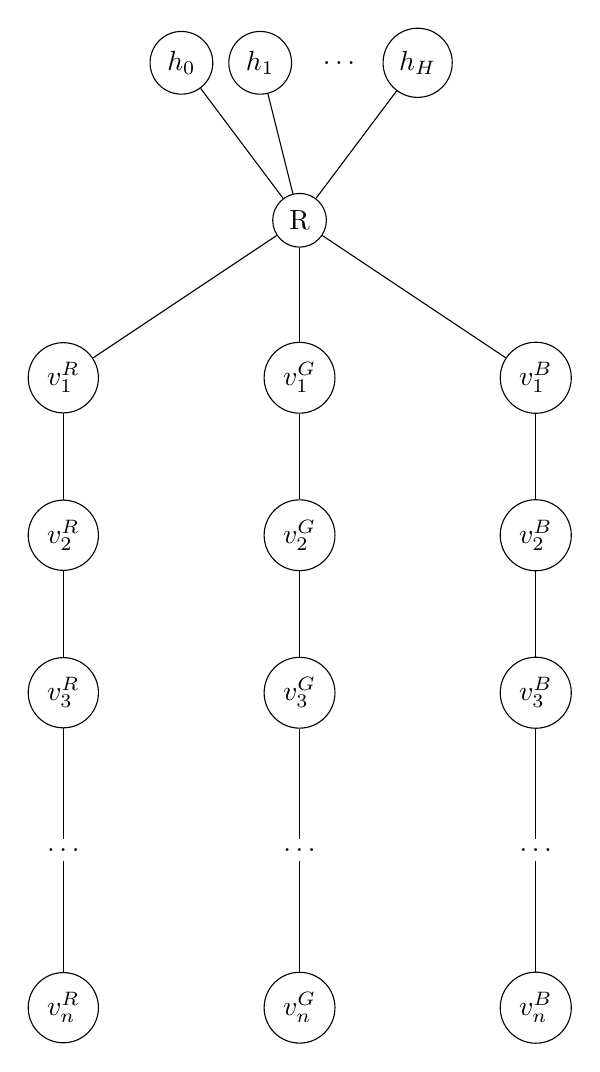
\begin{tikzpicture}
  \node[shape=circle,draw=black] (R) at (0,0) {R};
  \node[shape=circle,draw=black] (h1) at (-1.5,2) {$h_0$};
  \node[shape=circle,draw=black] (h2) at (-0.5,2) {$h_1$};
  \node (dots) at (0.5,2) {$\ldots$};
  \node[shape=circle,draw=black] (hH) at (1.5,2) {$h_H$};
  \node[shape=circle,draw=black] (v1R) at (-3,-2) {$v_1^R$};
  \node[shape=circle,draw=black] (v1G) at (0,-2) {$v_1^G$};
  \node[shape=circle,draw=black] (v1B) at (3,-2) {$v_1^B$};
  \node[shape=circle,draw=black] (v2R) at (-3,-4) {$v_2^R$};
  \node[shape=circle,draw=black] (v2G) at (0,-4) {$v_2^G$};
  \node[shape=circle,draw=black] (v2B) at (3,-4) {$v_2^B$};
  \node[shape=circle,draw=black] (v3R) at (-3,-6) {$v_3^R$};
  \node[shape=circle,draw=black] (v3G) at (0,-6) {$v_3^G$};
  \node[shape=circle,draw=black] (v3B) at (3,-6) {$v_3^B$};
  \node (dotsR) at (-3,-8) {$\ldots$};
  \node (dotsG) at (0,-8) {$\ldots$};
  \node (dotsB) at (3,-8) {$\ldots$};
  \node[shape=circle,draw=black] (vnR) at (-3,-10) {$v_n^R$};
  \node[shape=circle,draw=black] (vnG) at (0,-10) {$v_n^G$};
  \node[shape=circle,draw=black] (vnB) at (3,-10) {$v_n^B$};

  \path (R) edge node {} (h1);
  \path (R) edge node {} (h2);
  \path (R) edge node {} (hH);
  \path (R) edge node {} (v1R);
  \path (R) edge node {} (v1G);
  \path (R) edge node {} (v1B);
  \path (v1R) edge node {} (v2R);
  \path (v1G) edge node {} (v2G);
  \path (v1B) edge node {} (v2B);
  \path (v2R) edge node {} (v3R);
  \path (v2G) edge node {} (v3G);
  \path (v2B) edge node {} (v3B);
  \path (v3R) edge node {} (dotsR);
  \path (v3G) edge node {} (dotsG);
  \path (v3B) edge node {} (dotsB);
  \path (dotsR) edge node {} (vnR);
  \path (dotsG) edge node {} (vnG);
  \path (dotsB) edge node {} (vnB);

\end{tikzpicture}
\caption{Scaffolding tree $T_S$ in \tr reduction}
\label{q4:scaffolding}
\end{figure}


\begin{figure}
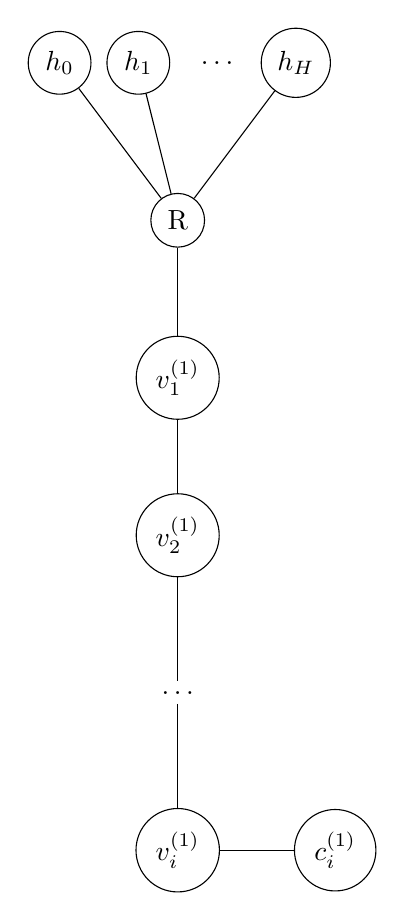
\begin{tikzpicture}
  \node[shape=circle,draw=black] (R) at (0,0) {R};
  \node[shape=circle,draw=black] (h1) at (-1.5,2) {$h_0$};
  \node[shape=circle,draw=black] (h2) at (-0.5,2) {$h_1$};
  \node (dots) at (0.5,2) {$\ldots$};
  \node[shape=circle,draw=black] (hH) at (1.5,2) {$h_H$};
  \node[shape=circle,draw=black] (v1) at (0,-2) {$v_1^{(1)}$};
  \node[shape=circle,draw=black] (v2) at (0,-4) {$v_2^{(1)}$};
  \node (dots1) at (0,-6) {$\ldots$};
  \node[shape=circle,draw=black] (vi) at (0,-8) {$v_i^{(1)}$};
  \node[shape=circle,draw=black] (ci) at (2,-8) {$c_i^{(1)}$};

  \path (R) edge node {} (h1);
  \path (R) edge node {} (h2);
  \path (R) edge node {} (hH);
  \path (R) edge node {} (v1);
  \path (v1) edge node {} (v2);
  \path (v2) edge node {} (dots1);
  \path (dots1) edge node {} (vi);
  \path (vi) edge node {} (ci);

\end{tikzpicture}
\caption{Vertex gadget tree $T_{v_i}$ in \tr reduction for vertex $v_i$}
\end{figure}

\begin{figure}
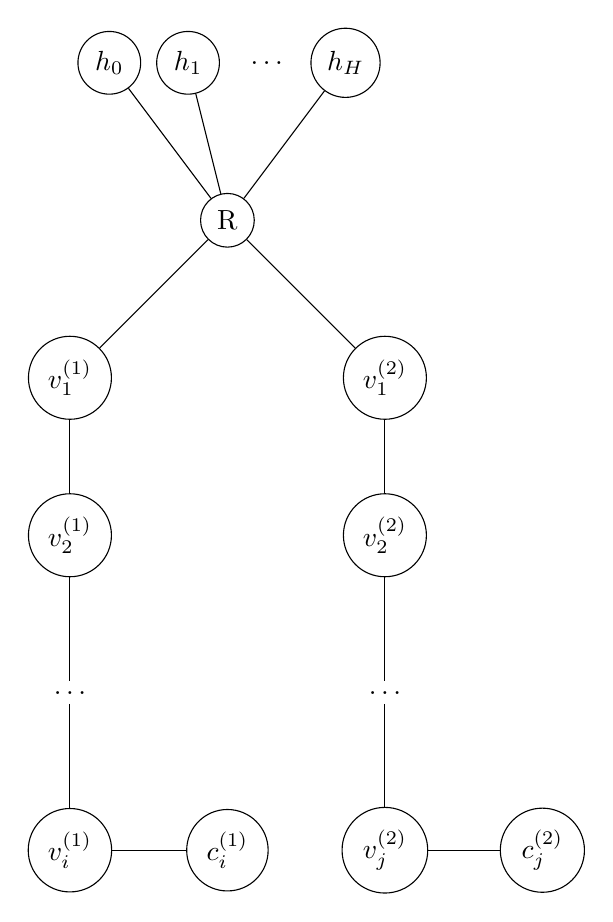
\begin{tikzpicture}
  \node[shape=circle,draw=black] (R) at (0,0) {R};
  \node[shape=circle,draw=black] (h1) at (-1.5,2) {$h_0$};
  \node[shape=circle,draw=black] (h2) at (-0.5,2) {$h_1$};
  \node (dots) at (0.5,2) {$\ldots$};
  \node[shape=circle,draw=black] (hH) at (1.5,2) {$h_H$};
  \node[shape=circle,draw=black] (v11) at (-2,-2) {$v_1^{(1)}$};
  \node[shape=circle,draw=black] (v12) at (2,-2) {$v_1^{(2)}$};
  \node[shape=circle,draw=black] (v21) at (-2,-4) {$v_2^{(1)}$};
  \node[shape=circle,draw=black] (v22) at (2,-4) {$v_2^{(2)}$};
  \node (dots1) at (-2,-6) {$\ldots$};
  \node (dots2) at (2,-6) {$\ldots$};
  \node[shape=circle,draw=black] (vi1) at (-2,-8) {$v_i^{(1)}$};
  \node[shape=circle,draw=black] (vj2) at (2,-8) {$v_j^{(2)}$};
  \node[shape=circle,draw=black] (ci1) at (-0,-8) {$c_i^{(1)}$};
  \node[shape=circle,draw=black] (ci2) at (4,-8) {$c_j^{(2)}$};

  \path (R) edge node {} (h1);
  \path (R) edge node {} (h2);
  \path (R) edge node {} (hH);
  \path (R) edge node {} (v11);
  \path (R) edge node {} (v12);
  \path (v11) edge node {} (v21);
  \path (v12) edge node {} (v22);
  \path (v21) edge node {} (dots1);
  \path (v22) edge node {} (dots2);
  \path (dots1) edge node {} (vi1);
  \path (dots2) edge node {} (vj2);
  \path (vi1) edge node {} (ci1);
  \path (vj2) edge node {} (ci2);

\end{tikzpicture}
\caption{Edge gadget tree $T_{(v_i,v_j)}$ in \tr reduction for edge $(v_i, v_j)$}
\end{figure}
